\cotefile{45}
\scanpage{33}\mspage{22}
% archive sheet number: 32
n\textsuperscript{o} 246

la réunion de $]\Delta_1,\Delta_2[$, de $\Delta_1$ et de $\Delta_2$.

\uline{Lorsque} $k$ \uline{satisfait à l'hypothèse du chapeau du n}\textsuperscript{o} 6, on peut, au moyen d'une forme quadratique auxiliaire, établir une correspondance biunivoque \uline{croissante} entre le corps $k$ et l'ensemble ordonné défini par la prop. 6. [N.B. Pour le cas où $k$ ne satisfait pas à l'hypothèse en question, l'adjudant de service fabriquera un contre-exemple et le mettra en exercice]. Pour cela, on introduit dans le plan $E$ n'importe quelle forme quadratique $\phi$ pour laquelle $-\delta$ est un carré, ce qui nous permet d'appliquer tous les résultats des n\textsuperscript{os} précédents. Pour toute demi-droite $\Delta$ autre que $\Delta_{\unsure{o|0}}$, on posera

\[
t(\Delta)=\operatorname{tg}\frac{1}{2}\,(-\Delta_o,\Delta).
\]

Comme on a $\Delta\ne\Delta_o$, $(-\Delta_o,\Delta)$ n'est pas l'angle plat, donc $\frac{1}{2}\,(-\Delta_o,\Delta)$ n'est pas un angle droit et par suite $t(\Delta)\ne\infty$. Il est immédiat que $\Delta\longrightarrow t(\Delta)$ est une bijection de l'ensemble des demi-droites $\ne\Delta_o$ sur $k$. On va montrer que cette bijection est croissante. Soient en effet $\Delta_1,\Delta_2$ deux demi-droites distinctes de $\Delta_o$ ; soit $t_i=t(\Delta_i)\quad(i=1,2)$\unsure{.} Soit $a$ un point, autre que $0$, sur $-\Delta_o$ ; pour la base $(a,Ja)$ de $E$, les demi-droites $\Delta_o,\Delta_1,\Delta_2$ contiendront respectivement (en vertu de la formule (12)) les points :

\[
\begin{aligned}
x_o&=(-1,0)\,,\\
x_i&=(1-t_i^2,\,2t_{\unsure{i|1}})\quad(i=1,2),
\end{aligned}
\]

Pour que la suite $\Delta_o,\Delta_1,\Delta_2$ soit directe, il faut et il suffit que deux au moins des quantités

\[
-2t_1,\quad(1-t_1^2)2t_2-(1-t_2^2)2t_1\,,\quad 2t_2
\]

soient $>0$. Or la seconde s'écrit $2(t_2-t_1)\,(1+t_1t_2)$.
\scanpage{34}
% archive sheet number: 33
% At far right a sliver of the leaf beneath bears a partial A-shaped mark.
Soit $G$ un \inserted{schéma en} groupe affine sur $A$, $A$-simple

\[
\begin{aligned}
\operatorname{Aff}_A(G)&\qquad\text{son algèbre affine}\\
\mathcal U_A(G)&\qquad\text{son hyperalgèbre}
\end{aligned}
\]

Donc $\deleted{\unsure{\{|\ell}}$ $\operatorname{Aff}_A(G)$ est une $A$-algèbre commutative augmentée, munie d'un \unsure{hom|homom.} diagonal multiplicatif, associatif, compatible avec les augmentations

$U_A(G)$ est une $A$-algèbre en général non comm., munie d'un hom diagonal multiplicatif, associatif, comm. compatible avec les augmentations

Il y a un produit scalaire

\[
\langle f,X\rangle=\langle\deleted{\unsure{f}}X,\deleted{\unsure{X}}f\rangle
\]

entre $\operatorname{Aff}_A(G)$ et $U_A(G)$, ce dernier s'identifiant aux formes $A$-linéaires sur $\operatorname{Aff}_A(G)$ qui s'annulent sur une puissance de l'idéal d'augmentation

$U_A(G)$ opère à g. et à droite sur $\operatorname{Aff}_A(G)$ [qui est un bimodule sur $U_A(G)$]

\[
\left\{\begin{aligned}
\langle Y,X*f\rangle&=\langle Y*X,f\rangle=\langle f,Y*X\rangle=\langle f*Y,X\rangle\\
\langle\varepsilon,X*f\rangle&=\langle\varepsilon,f*X\rangle=\langle X,f\rangle
\end{aligned}\right.
\]
\scanpage{35}
% archive sheet number: 34
$\operatorname{Aff}_A(G)$ opère \deleted{à gauche et à droite} sur $U_A(G)$ ; \unsure{les formules sont|la formule est} \deleted{\unsure{de façon|de la façon|transposée}} \unsure{analogues|analogue}

\[
\langle g,f\mathbin{\lrcorner}X\rangle=\langle gf,X\rangle
\qquad\text{en particulier}\quad\langle f,X\rangle=\varepsilon(f\mathbin{\lrcorner}X)
\]

Supposons maintenant que $A\subset B$, alors

\[
\operatorname{Aff}_B(G)=\operatorname{Aff}_A(G)\otimes_A B\supset\operatorname{Aff}_A(G)
\]

[on a une \uline{inclusion}, car $\operatorname{Aff}_A(G)$ plat sur $A$]

\[
U_B(G)=U_A(G)\otimes_A B\supset U_A(G)
\]

[raison analogue ; la première égalité est due au fait que $G$ est $A$-simple]

\uline{Proposition 1}\quad Soit $X\in U_B(G)$. Conditions équivalentes

\[
\begin{aligned}
\text{(i)}\quad &X\in U_A(G)\\
\text{(ii)}\quad &X*\operatorname{Aff}_A(G)\subset\operatorname{Aff}_A(G)
  \qquad\text{(ii bis)}\quad\operatorname{Aff}_A(G)*X\subset\operatorname{Aff}_A(G)\\
\text{(iii)}\quad &\langle X,\operatorname{Aff}_A(G)\rangle\subset A
\end{aligned}
\]

En effet,

\diagram{\begin{tikzcd}[ampersand replacement=\&,column sep=small,row sep=tiny]
\& \text{(ii bis)}\arrow[dr,Rightarrow] \& {}\\
\text{(i)}\arrow[ur,Rightarrow]\arrow[r,Rightarrow] \& \text{(ii)}\arrow[r,Rightarrow] \& \text{(iii)}
\end{tikzcd}}

triviaux.

(iii) implique que \deleted{$X\unsure{\in|\mathbin{\lrcorner}}\operatorname{Aff}$} \deleted{la forme} \inserted{$X$ \unsure{définit|est}} une forme $A$-linéaire sur $\operatorname{Aff}_A(G)$ nulle sur une puissance de l'idéal d'augmentation, donc un élément $X_{\unsure{0|o}}$ de $U_A(G)$, qui n'est évidemment autre que $X$
\scanpage{36}
% archive sheet number: 35
\uline{Proposition 2}\quad Soit $f\in\operatorname{Aff}_B(G)$\deleted{\unsure{supposons}}\inserted{Supposons $G$ $A$-connexe}. Conditions équivalentes

\margin{$\unsure{X})$}

\[
\begin{aligned}
\text{(i)}\quad &f\in\operatorname{Aff}_A(G)\\
\text{(ii)}\quad &f\mathbin{\lrcorner} U_A(G)\subset U_A(G)\\
\text{(iii)}\quad &\langle f,U_A(G)\rangle\subset A
\end{aligned}
\]

Évidemment $\text{(i)}\Rightarrow\text{(ii)}\Rightarrow\text{(iii)}$ [\unsure{de|et} $\text{(}\deleted{\unsure{\mathrm{ii}}}\mathrm{iii}\text{)}\Rightarrow\text{(ii)}$ car \deleted{\unsure{soit}} $X\in U_A(G)$, pour prouver $f\mathbin{\lrcorner}X\in U_A(G)$ il suffit \inserted{(prop. 1)} de vérifier que $\langle g,f\mathbin{\lrcorner}X\rangle\in A$ pour $g\in\operatorname{Aff}_A(G)$, or $\langle g,f\mathbin{\lrcorner}X\rangle=\langle gf,X\rangle=\langle f,g\mathbin{\lrcorner}X\rangle\in\langle f,U_A(G)\rangle\subset A$] Prouvons $\text{(iii)}\Rightarrow\text{(i)}$ en utilisant que $G$ est $A$-connexe.

Soit $C\deleted{B}=\operatorname{Aff}_A(G)$, considérons le diagramme

\diagram{\begin{tikzcd}[ampersand replacement=\&]
C\arrow[r]\arrow[d,very thick] \& C_B\arrow[d]\\
\widehat C\simeq\operatorname{Hom}_A(U,A)\arrow[r] \& \widehat C_B=\operatorname{Hom}_B(U_B,B)
\end{tikzcd}}

où $\widehat{\phantom C}$ désigne le \inserted{\unsure{séparé}} complété pour l'idéal d'augmentation.
\scanpage{37}
% archive sheet number: 36
Cohomologie de l'algèbre de Lie et \unsure{coh.|ob.|cohom.} \unsure{du|des} \unsure{groupe|groupes} \ldots
\scanpage{38}
% archive sheet number: 37

Soit \(G\) un schéma en groupes simple sur \(S=\operatorname{Spec} A\), \(A\) Artinien local.

\[
\mathfrak g=L_S(G)
\]

(1) Si \(H^0(\mathfrak g_0,\mathfrak g_0)=0\), \deleted{\unsure{alors}}\(\Longleftrightarrow\) \(G\longrightarrow\underline{\operatorname{Aut}}_S(\mathfrak g)\) est \deleted{\unsure{\illegible{1}|un}} non ramifié

[donc si \(G_0\) n'a pas de sous-groupe \deleted{discret} étale \deleted{\unsure{forcément|forcément un}} non trivial, alors c'est une imm. fermée]

(2) \deleted{Si}\inserted{(1) et} \inserted{\deleted{de plus}} \(H^1(\mathfrak g_0,\mathfrak g_0)=0\) \deleted{\unsure{alors}}\(\Longleftrightarrow\) \(G\longrightarrow\underline{\operatorname{Aut}}_S(\mathfrak g)\) est étale,

[donc sous la condition dite plus haut, c'est une imm. ouverte, donc \deleted{\unsure{Aut}}\(G\simeq\underline{\operatorname{Aut}}_S^{\circ}(\mathfrak g)\) \deleted{\unsure{G}}si \(G\) à fibres connexes]

% slanted
\margin{\deleted{(1) et (2)} (2) \(\Longrightarrow\) \(\underline{\operatorname{Aut}}_S(\mathfrak g)\simeq\underline{\operatorname{Aut}}_S(G)\) si \(G\) connexe \ldots\ Utilisant \unsure{Tchoka|Tôhoku|Tohoku}, cela suffirait à construire les \unsure{Tchokas|Tôhokus|Tohoku} \deleted{\illegible{1}} sur \(Z\) \ldots}

Supposons qu'on ne dispose pas de \(G\), mais seulement de \(\mathfrak g\), considérons \(H=\underline{\operatorname{Aut}}_S(\mathfrak g)\). \deleted{Alors} C'est un schém. en groupes sur \(S\), et \(\operatorname{Lie}_k(H_0)=\mathfrak h_0\) est isomorphe à \deleted{\(\mathfrak g_0/(\text{centre de }\mathfrak g_0)\) par \unsure{iso. canonique|son caractère|iso}} \inserted{l'Algèbre de Lie des} dérivations de \(\mathfrak g_0\), d'où \(\mathfrak g_0\to\mathfrak h_0\), qui est un isom. si (1) et (2) sont satisfaites.

S'il en est ainsi, on ne peut affirmer encore que \deleted{\unsure{G}}\(H\) est simple sur \(S\), \unsure{\(=\)|\(\simeq\)} le long de la section unité, \deleted{Mais dans} \unsure{On|Or} le peut si on suppose

\[
\text{(3)}\qquad H^2(\mathfrak g_0,\mathfrak g_0)=0
\]

qui signifie sauf erreur qu'il n'y a pas de \unsure{variation|variations} de structure \inserted{\unsure{infinitésimales|infinitésimale}} non triviales de \(\mathfrak g_0\), et \uline{implique} que \deleted{\unsure{les deux|tous deux}} \(\underline{\operatorname{Aut}}_S(\mathfrak g)\) est simple sur \(S\).
\scanpage{39}
% archive sheet number: 38

que toute fonction rationnelle definie en \(x\) soit definie en \(y\). \deleted{Alors \(\underline O_y\) \unsure{domine}} La condition est de toutes façons necessaire, prouvons qu'elle est suffisante (utilisant la separation). Supposons \(\underline O_x\quad\underline O_y\), donc (\deleted{\unsure{l}}lem\deleted{\unsure{l}}me 1) il existe un ideal premier \(\underline p\)\deleted{\unsure{n}}de \(\underline O_x\) tel que \(\underline O_y\) domine \(\underline O_{x\,\underline p}\). Or il existe un \(z\quad X\) tel que \(x\quad\bar z\), \(\underline O_z=\underline O_{x\,\underline p}\) (reference
% The right edge cuts the type at this word.
donc \(\underline O_z\) et \(\underline O_y\) sont apparentes, donc \(z=y\) cqfd.

On peut reenoncer ce corollaire ainsi: si \(x\unsure{\notin|\ne}\bar y\), il existe une fonction rationnelle \(f\) sur \(X\) telle que \(f\) soit definie en \(x\) et non en \(y\) i.e. telle que \(D(f)\) contienne \(x\) et ne rencontre pas \(\bar y\). Si maintenant \(X\) est un espace noetherien, toute partie fermee de \(X\) est reunion finie de fermes irreductibles, i.e. de la forme \(\bar y\), d'ou:

\uline{Corollaire} 3 Soit \(X\) un schema integre noetherien (il suffit de dire: qui est un espace topologique noeth.), alors les \(D(f)\) forment une base de la topologie de \(X\).

On voit ainsi comment la topologie de \(X\), identifie a un ensemble de sous-anneaux locaux de \(R\), peut se recuperer en termes de cette derniere structure; de façon equivalente, on peut aussi remarquer que la topologie de \(X\) est definie entermes de sa structure d'ordre, un ferme de \(X\) etant forme des elements de \(X\) majores par un au moins parmi les elements d'une partie finie de \(X\) (la majoration etant definie \deleted{\unsure{soit|sut}} ici en termes d'inclusions \deleted{de parties \unsure{irre|irra}} d'anneaux locaux). D'autre part, le faisceau \(\underline O_X\) lui aussi est recupere, puisque

\[
I\ (U,\underline O_X)=\quad\underline O_x\ (x\quad U)
\]

Plus bas, nous donnerons quelques indications plus precis\deleted{\unsure{s|x}}es.

\uline{Proposition} 3 Soit \(f:X\quad Y\) un morphisme dominant de schemas integres, \deleted{\unsure{de cor|du cor}} soit \(L\) (\(K\)) le corps de \(X\) (\(Y\)). Identifions \(K\) a un sous-corps de \(L\), et les anneaux locaux de \(X\) (\(Y\)) a des sous-anneaux de \(L\) (\(K\)). Alors pour tout \(x\quad X\), \(\underline O_{f(x)}\) est l'unique anneau local de \(Y\) domine par \(\underline O_x\).

Il est en effet domine, par definition d'un morphisme, et il est unique puisque deux anneaux locaux de \(Y\) apparentes sont identiques.

\uline{Proposition} 4 Soit \(f\) un morphisme \uline{separe} d'immersion locale (resp. d'isomorphisme local) de \(X\) dans \(Y\), avec \deleted{\(Y\)} \(X\) \uline{irreductible}. Alors \(f\) est une immersion (resp. une immersion ouverte).

Il suffit de montrer que \(f\) est un homeomorphisme dans (ce qui impliquera facilement, compte tenu de l'hypothese, que \(f(X)\) est localement ferme dans \(Y\)). On peut evidemment supposer \(X\) et \(Y\) \uline{reduits}, et on voit qu'on peut remplacer \(Y\) par l'adherence de \(f(X)\), donc on peut supposer \(f\) dominant. Alors \deleted{\(Y\) sera aussi \unsure{in|ir}} \(Y\) sera aussi irreductible, donc \(X\) et \(Y\) sont integres. Avec les notations de prop.3, on aura pour tout \(x\quad X\)
\scanpage{40}
% archive sheet number: 39

De plus, (1) (2) (3) [\unsure{impliquent|implique|l'idée que} l'existence d'un \(G\) \deleted{\unsure{de}}\unsure{simple} sur \(S\) donnant \(\mathfrak g\)] prouvent aussi [pour \(G\) connexe] que \(G_{\unsure{\bullet|0}}\) n'a pas de variations infinitésimales non triviales.

Question de relèvement de la structure \(G\)\inserted{ (\(G\) connexe)}, équivaut à la question de relèvement de la structure \(\mathfrak g\). On trouve une obstruction dans \(H^3(\mathfrak g,\mathfrak g)\). Donc

\deleted{\(H^{3}\)}

(3) Si \(H^3(\mathfrak g,\mathfrak g)=0\), alors on peut relever de façon \unsure{essentiellt|essentiellement} unique \(\mathfrak g\), ou \(G\) de façon équivalente.

\uline{Question} Définir \(H^{\unsure{*|\alpha}}(G,\mathfrak g)\to H^*(\mathfrak g,\mathfrak g)\)

[plus généralement, si on a une représentation linéaire de \(G\) \ldots]. Suite spectrale reliant \(H^*(G,\ )\) et \(H^*(\mathfrak g,-)\) ?? Elle exprimerait la \textquotedblleft différence\textquotedblright\ entre le global, et l'infinitésimal.

Supposons \(G\) semi-simple adjoint. A-t-on alors

\[
H^*(\unsure{G|h},\mathfrak g)=H^*(\mathfrak g,\mathfrak g)=0\qquad ??
\]
\scanpage{41}
% archive sheet number: 40

Soit \(X\) un\deleted{p} preschema \uline{integre}, soit \(R\) son corps des fonctions rationnelles (anneau local de l'element generique). Pour tout \(x\quad X\), \deleted{\(\underline O\)} l'anneau local \(\underline O_{\deleted{\unsure{X}}x}\) est integre et a \(R\) comme corps des frac\deleted{\unsure{o|b}}tions, donc \(\underline O_x\) s'identifie a un sous-anneau de \(R\). Si \(f\quad R\), on dit que \(f\) est \uline{definie en} \(x\) si \(f\quad\underline O_x\), et l'ensemble des \(x\quad X\) ou \(f\) est definie est appele le \uline{domaine de definition} de \(f\), note \(D(f)\) (?). Il est evidemment \uline{ouvert}. Si \(U\quad X\) est ouvert, on a \(I\ (U,\underline O_X)=\quad\underline O_x\quad(x\quad U)\)

\uline{Proposition} 2 Soient \(X\) un pres\deleted{\unsure{e}}chema integre de corps des fractions \(R\). Pour que \(X\) soit un schema, il faut et il suffit que pour tout couple de points \(x,y\quad X\), \(\deleted{\unsure{D}}\underline O_x\) et \(\underline O_y\) apparentes implique \(x=y\).

Supposons cette condition verifiee, montrons que \(X\) est separe. Soient \(U\) et \(V\) deux ouverts affines de \(X\), \(A\) et \(B\) leurs anneaux, identifies a des sous-anneaux de \(R\). L'hypothese implique que \(A\) et \(B\) sont non apparentes (cf prop.1), \deleted{dans \(S(A)\quad S(B)\)} et \(U\) (\(V\)) s'identifie a \(S(A)\) (\(S(B)\)), alors \(U\ V\) s'identifie a \(S(A)\ S(B)=S(C)\), ou \(C\) est l'\deleted{\unsure{annea|anneau}} l'anneau engendre par \(A\) et \(B\) dans \(R\). D'ailleurs, \(C\) est identique a l'intersection des \(Q\quad S(C)\), donc s'identifie a \(I\ (U\ V,\underline O_X)\). Soit \(W=U\ V\), c'est un preschema tel que, posant \(C=I\ (W,\underline O_W)\), le morphisme naturel \(W\quad\operatorname{Spec}(C)\) deduit de \(C\quad I\ (W,\underline O_W)\) soit bijectif (au point de vue ensembliste). Il s'ensuit facilement ici que c'est un homeomorphisme, car tout ferme de \(W\) est la trace de son adherence dans \(U\), donc defini par un ideal de \(A\) et a fortiori par un ideal de \deleted{\unsure{,|y}} \(C\), donc est l'image reciproque d'un ferme de \(\operatorname{Spec}(C)\). On voit de meme qu'on a \deleted{\unsure{u}}en fait un \uline{isomorphisme} de preschemas, i.e. des isomorphismes pour les anneaux locaux. Donc \(U\ V\) est affine, d'autre part son anneau \(C\) est engendre par les anneaux \(A\) et \(B\) de \(U\) et \(V\). Cela prouve que \(X\) est separe (refernce).

Inversement, supposons \(X\) separe, soient \(x,y\quad X\) tels que \(\underline O_x\) et \(\underline O_y\) soient apparentes. Soit \(U\) (\(V\)) un voisinage affine de \(x\) (\(y\)) d'anneau \(A\) (\(B\)), alors \(U\ V\) est affine d'anneau l'anneau \(C\) engendre par \(A\) et \(B\) (meme reference). \deleted{En vertu de prop 1, dont la} Alors \(x\)\inserted{ (\(y\))} correspond a un ideal premier \(\underline p\) (\(\underline q\)) de \(A\) (\(B\)), et comme \deleted{\(Ap\)} \(A_{\underline p}\) et \(B_{\underline q}\) sont apparentes il existe un ideal premier \(\underline r\) de \(C\) induisant \(\underline p\) et \(\underline q\). Alors \(\underline r\) correspond a un point \(z\) de \(U\ V\), et on a evidemment \(x=z\) et \(y=z\), d'ou \(x=y\).

\uline{Corollaire} 1 Si \(X\) est un schema integre, l'application \(x\quad\underline O_x\) est un monomorphisme, i.e. si \(x\) et \(y\) sont des points distincts de \(X\), alors il existe un fonction rationnelle definie en l'un et non en l'autre.

De façon plus precise:

\uline{Corollaire} 2 Soit \(X\) un schema integre, soient \(x,y\) deux points de \(X\). Pour qu'on ait \(x\quad\bar y\) i.e. \(\bar x\quad\bar y\), il faut et il sffit que \(\underline O_x\quad\underline O_y\), ie.
\scanpage{42}
% archive sheet number: 41

\[
X\qquad Y\qquad H
\]

\[
\left\{\begin{aligned}
[X,H]&=\lambda(H)X\\
[Y,H]&=-\lambda(H)Y\\
[X,Y]&=H
\end{aligned}\right.
\]

\diagram{\begin{tikzcd}[ampersand replacement=\&,column sep=small,row sep=small]
{} \arrow[d] \& {} \& {}\\
{} \& T\arrow[r] \& T'\\
{} \& \unsure{\mu_2|p_2} \& {}
\end{tikzcd}}

\[
\deleted{[X,H]}\qquad \mathcal U\subset
\]

\uuline{\(\unsure{\operatorname{Sp}|\operatorname{SP}|\operatorname{Sl}}(2)\)}

\unsure{Groupe|Gpe|Groupes} \deleted{\unsure{projectif|projector|proches}} \unsure{racinaire|réductifs} \(=\) groupe \unsure{de dim un|de dimension un|quel cas}.

\figure{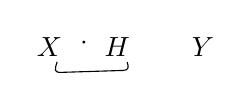
\begin{tikzpicture}[x=1em,y=1em,baseline=0pt]
\node at (0,0) {\(X\)}; \node at (1.25,0.16) {\(\cdot\)}; \node at (2.45,0) {\(H\)}; \node at (5.55,0) {\(Y\)};
\draw (0.28,-0.52) .. controls (0.17,-0.83) and (0.18,-0.90) .. (0.42,-0.90) -- (2.65,-0.83) .. controls (2.87,-0.82) and (2.87,-0.73) .. (2.81,-0.53);
\end{tikzpicture}}

\[
[X,Y]=0
\]

Algèbre de Lie de \(\operatorname{Sl}(2,k)\) \hfill Car \(2\).

\[
\deleted{[X,H]=\lambda\unsure{1|(}}
\]

\[
\left\{\begin{aligned}
[H,X]&=\deleted{\unsure{\lambda(H)X|2X}}\,0\\
[H,Y]&=\deleted{\unsure{-2Y|-Y}}\,0\\
[X,Y]&=H
\end{aligned}\right.\qquad\qquad \mathcal U
\]

Normalisateur de \(k.\deleted{\unsure{X}}Y=\mathcal U\) est \(k.Y+k.H=\mathscr L\)

Normalisateur de \(k.H=\unsure{\mathfrak h|\mathfrak g_a}\) est \(\mathfrak g\) tt. entier

Algèbre de Lie de \(\deleted{\unsure{S}}\unsure{\operatorname{Pl}|\operatorname{PGl}|\operatorname{SPl}|\operatorname{Spl}}(2,k)\).

\[
\left\{\begin{aligned}
[H',X]&=X\\
[H',Y]&=-Y\\
[X\unsure{.|,}Y]&=0
\end{aligned}\right.
\]

Normalisateur de \(k.Y\) est \(\mathfrak g\)

Normalisateur de
\scanpage{45}
% archive sheet number: 44
\uline{Formes extérieures types}

\margin{\(\deleted{E_0=\operatorname{Ext}(G_0)}\quad H_0=\operatorname{ad}(G_0)\)}

\(G_0\) un groupe \(\tfrac12\) simple type (sur \(Z\)), \(\Gamma_0=\underline{\operatorname{Aut}}_Z(G_0)\), \deleted{\(\unsure{E=E/E^\circ|\Gamma=\Gamma/\Gamma^\circ}\)}, on a \deleted{\(\unsure{E\rtimes|E H}\)}\inserted{\(\Gamma_0\simeq E_0 H_0\)}

\(E_0\) sous-groupe \unsure{conservant|normalisant} \(T_0\subset B_0\)

\(S\) schéma de base

\(G\) forme de \(G_0\) sur \(S\), correspond : un principal \unsure{homogène|hom.} \deleted{\(\unsure{P_G|Q_G|P}\)}\inserted{\(\unsure{Q_0|P_0}\)} sous \(\Gamma_S\), \deleted{\illegible{1}} \deleted{\(\unsure{Q_G|P_G|P}\)}\inserted{\(\unsure{P|\rho}=P_G\)} le principal homogène associé de groupe \(E\), \deleted{qui} est \unsure{parfois|partie|noté} par abus de langage l'élément correspondant de \(H^1(S,E_0)\).

\inserted{\deleted{\unsure{plus précisément} \(\unsure{G_0^P|G^P}\)}}

\(G_1=G_0^P\) déduit de \(G_0\) en tordant par \(P\)\inserted{ [pour l'instant, \unsure{par hypoth.|par not.} \(P=P_G\)]} : une telle \deleted{groupe} forme \unsure{sera|ser.} dite \uline{forme extérieure type} associée à \(P\).

[On dit que \(G\) est une forme extérieure type s'il est \uline{isom.} à \(G_{1}^{\unsure{P|*|\rho}}\), \deleted{\unsure{tel}} \deleted{\unsure{si|et}} \unsure{nécessairemt|nécessairement} \(P\simeq P_G\)]

Si on part de \(P\), [sans \(G\)], \uline{la donnée d'un \(G\) et d'un} \uline{isom} \(\deleted{\unsure{G}}P\mathrel{\overset{\varphi}{\overset{\sim}{\longrightarrow}}}\deleted{\unsure{G}}P_G\) \textquotedblleft\uline{équivaut}\textquotedblright\ \uline{à la donnée d'un fibré principal homogène sous} \(H_1=\deleted{\unsure{G}}H_0^P\) ; la

% slanted
\margin{Distinguer entre les tores maximaux de \(G_0\) et \(H_0\), de \unsure{de|dans} \(G_1\) et \(H_1\), \ldots}

Classification des objets \(G\) à isom. près : [un isom de \((G,\varphi)\) et \((G',\varphi')\) étant donné : un isom \(\psi:G\to G'\) tel que l'isom correspondant \(P_G\xrightarrow{\sim}P_{G'}\) soit compatible avec les isom \(P_G\) et \(P_{G'}\) avec \(P\) \unsure{fixé|fix.} ; \uline{un tel} \deleted{\unsure{cet iso|cette}} \uline{isomorphisme est dit} \uline{intérieur}] \deleted{revient} \deleted{à \unsure{classifiant|classification}} est donnée par \(H^1(S,\deleted{\unsure{G}}H_{1}^{\unsure{P|1}})\). On a

% slanted
\margin{Définir ainsi la notion d'isom. \uline{\unsure{intérieur|extérieur}} d'un \unsure{gpe en lui-même|groupe en lui-même}.}

\[
H^1(S,\deleted{\unsure{G}}H_1^{\unsure{P|1}})\longrightarrow H^1(S,\Gamma)=\text{ens des classes \unsure{à isom|d'isom}}
\]

près de formes de \(G\) sur \(S\)

\(\text{\textquotedblright}\) \unsure{ens|ensemble|son} des classes : isom près de \textquotedblleft formes \deleted{relatives} intérieures relatives à \(P\)\textquotedblright
\scanpage{46}\mspage{73}
% archive sheet number: 45
n\textsuperscript{o} 239

\S\,4. \uline{Prolongement de sections}. \uline{Faisceaux fins}

1. \uline{Sections d'un faisceau déduit d'un préfaisceau}.

Soient \((\mathscr F_U,\rho_{VU})\) un préfaisceau sur un espace \(X\), \(\mathscr F\) le faisceau qui s'en déduit. On a vu au \S\,1, n\textsuperscript{o}7 que, moyennant les conditions \((\mathrm{PF}_{\mathrm I}(U))\) et \((\mathrm{PF}_{\mathrm{II}}(U))\), supposées vérifiées pour tout \(U\in\Phi\) \uline{toute} section de \(\mathscr F\) au-dessus d'un ensemble \(U\in\Phi\) est de la forme \(x\longrightarrow\rho_{x,U}(f_U)\), où \(f_U\in\mathscr F_U\) (\S\,1, prop.14). Nous allons voir que dans certains cas la condition \((\mathrm{PF}_{\mathrm{II}}(U))\) à elle seule est suffisante pour qu'on puisse aboutir à cette conclusion :

PROPOSITION 1. -- \uline{Soient} \(X\) \uline{un espace topologique}, \((\mathscr F_U,\rho_{VU})\) \uline{un préfaisceau sur} \(X\) \uline{relatif à l'ensemble} \(\Phi\) \uline{de toutes les parties ouvertes de} \(X\), \(\mathscr F\) \uline{le faisceau déduit de ce préfaisceau}. \uline{Si} \(U\in\Phi\) \uline{est un sous-espace paracompact de} \(X\), \uline{et si la condition} \((\mathrm{PF}_{\mathrm{II}}(U))\) \uline{est satisfaite}, \uline{toute section de} \(\mathscr F\) \uline{au-dessus de} \(U\) \uline{est de la forme} \(x\longrightarrow\rho_{x,U}(f_U)\).

Nous démontrerons d'abord le lemme suivant :

LEMME 1. -- \uline{Soient} \(Y\) \uline{un espace normal}, \((U_\alpha)_{\alpha\in A}\) \uline{un recouvrement ouvert localement fini de} \(Y\). \uline{Pour tout couple d'indices} \(\alpha,\beta\) \uline{et tout} \(y\in U_\alpha\cap U_\beta\), \uline{supposons donné un voisinage ouvert} \(V_{\alpha\beta}(y)\) \uline{de} \(y\) \uline{contenu dans} \(U_\alpha\cap U_\beta\). \uline{Alors}, \uline{il existe une application} \(y\longrightarrow V(y)\) \uline{de} \(Y\) \uline{dans l'ensemble des parties ouvertes de} \(Y\), \uline{telle que pour tout} \(y\in Y\), \uline{on ait} \(y\in V(y)\), \uline{et que les conditions suivantes soient remplies} :

1) \uline{si} \(y\in U_\alpha\cap U_\beta\), \(V(y)\subset V_{\alpha\beta}(y)\) ;

2) \uline{si} \(y',y''\) \uline{sont tels que} \(V(y')\cap V(y'')\ne\phi\), \uline{il existe un} \(\alpha\) \uline{tel que} \(V(y')\cup V(y'')\subset U_\alpha\).

En effet, \((U_\alpha)\) étant un recouvrement localement fini et \(Y\) étant
\scanpage{47}
% archive sheet number: 46

la flèche \unsure{résulterait|résulte} aussi de la suite exacte de \unsure{S-groupes|groupes} sur \(S\)

\diagram{\begin{tikzcd}[ampersand replacement=\&,column sep=small]
e\arrow[r] \& \deleted{G}\unsure{\Gamma|H|\Pi}_1^{\deleted{\unsure{P|\rho}}}\arrow[r] \& \Gamma_1^{\deleted{P}}\arrow[r] \& E_1^{\deleted{P}}\arrow[r] \& e \& \Gamma_1^{\deleted{P}}\simeq E_1^{\deleted{P}}\,\deleted{G}\Gamma_1^{\deleted{P}}
\end{tikzcd}}

qui permet d'écrire

\diagram{\begin{tikzcd}[ampersand replacement=\&,column sep=small,row sep=small]
H^0(S,\deleted{\unsure{\Gamma}}E_1^{\deleted{P}})\arrow[r] \& H^1(S,\deleted{G}\Gamma_1^{\unsure{\circ|P|\rho}})\arrow[r] \& H^1(S,\Gamma_1^{\deleted{P}})\arrow[r]\arrow[d,equal] \& H^1(S,E^P)\\
{} \& {} \& H^1(S,\Gamma) \& {}
\end{tikzcd}}

\deleted{On a :} À priori, l'application envisagée n'est pas injective. \deleted{\unsure{Ainsi|Si}}\inserted{Cependant} l'\unsure{ens|un|ens.} des éléments \deleted{\unsure{qui}} de \(H^1(S,\Gamma_1^\circ)\) qui donnent l'élément neutre de \(H^1(S,\Gamma_1^{\deleted{P}})\) \deleted{\unsure{sont ceux qui|sont ceux que}} est en correspondance biunivoque avec \(H^0(S,E^P)/\deleted{\operatorname{Im}}H^0(S,\Gamma^P)\), est trivial puisque \(\Gamma_1^{\deleted{P}}\) est un produit \(\tfrac12\) direct.

Mais si \(\xi\in H^1(S,\deleted{G}\Gamma_1^\circ)\), on peut utiliser \(\xi\) pour tordre encore la situation, on trouve

\diagram{\begin{tikzcd}[ampersand replacement=\&,column sep=small,row sep=small]
e\arrow[r] \& (\deleted{G}\Gamma_1^{\deleted{P}})^\xi\arrow[r] \& (\Gamma_1^{\deleted{P}})^\xi\arrow[r]\arrow[d,equal] \& \deleted{(}E_1^{\deleted{P}}\deleted{)^\xi}\arrow[r] \& e\\
e\arrow[r] \& \operatorname{Ad}(G)\arrow[r] \& \operatorname{Aut}(G)\arrow[r] \& \operatorname{Ext}(G)\arrow[r] \& e
\end{tikzcd}}

et ici, on est ramené à la question si \deleted{\unsure{les|tout}} automorphisme ext. de \(G\) provient d'un automorphisme \(G\) n'est pas du tout évident quand \(G\) n'est \deleted{\unsure{autre chose que|pas un groupe}} pas une forme extérieure type. [i.e. \deleted{\unsure{on puisse|groupe}} n'ait \unsure{un|pas} de ss-groupe de Borel \(\supset\) Tore maximal].

% slanted
% enclosed in a pen oval
\margin{\uline{exemple} : sur un corps \unsure{à trouver|à Bra|de base} ??}

% slanted
\margin{Faux sur \(\mathbb R\) avec les formes \unsure{diverses|tordues} (\unsure{gpes unitaires|gpes unitaires en|gr. unitaires}): deux formes hermitiennes opposées donnent le \(=\) \unsure{gpe|groupe|gr.} Algébrique sur \(\mathbb R\) mais ne sont pas isom.}
